\documentclass[a4paper]{article}
\usepackage[T1]{fontenc}
\usepackage[utf8]{inputenc}
\usepackage[spanish]{babel}
\usepackage{mathtools}
\usepackage{amsmath}
\usepackage{graphics}
\usepackage{multicol}
\usepackage{listings}
\usepackage{color, colortbl}
\usepackage{amsfonts}

\newcommand{\HRule}{\rule{\linewidth}{0.5mm}}


\definecolor{mygreen}{rgb}{0,0.6,0}
\definecolor{mygray}{rgb}{0.5,0.5,0.5}
\definecolor{mymauve}{rgb}{0.58,0,0.82}

\definecolor{LightCyan}{rgb}{0.88,1,1}

\lstset{ %
	backgroundcolor=\color{white},   % choose the background color; you must add \usepackage{color} or \usepackage{xcolor}
	basicstyle=\footnotesize,        % the size of the fonts that are used for the code
	breakatwhitespace=false,         % sets if automatic breaks should only happen at whitespace
	breaklines=true,                 % sets automatic line breaking
	captionpos=b,                    % sets the caption-position to bottom
	commentstyle=\color{mygreen},    % comment style
	deletekeywords={...},            % if you want to delete keywords from the given language
	escapeinside={\%*}{*)},          % if you want to add LaTeX within your code
	extendedchars=true,              % lets you use non-ASCII characters; for 8-bits encodings only, does not work with UTF-8
	frame=single,                    % adds a frame around the code
	keywordstyle=\color{blue},       % keyword style
	language=C,                 % the language of the code
	morekeywords={*,...},            % if you want to add more keywords to the set
	numbers=left,                    % where to put the line-numbers; possible values are (none, left, right)
	numbersep=5pt,                   % how far the line-numbers are from the code
	numberstyle=\tiny\color{mygray}, % the style that is used for the line-numbers
	rulecolor=\color{black},         % if not set, the frame-color may be changed on line-breaks within not-black text (e.g. comments (green here))
	showspaces=false,                % show spaces everywhere adding particular underscores; it overrides 'showstringspaces'
	showstringspaces=false,          % underline spaces within strings only
	showtabs=false,                  % show tabs within strings adding particular underscores
	stepnumber=1,                    % the step between two line-numbers. If it's 1, each line will be numbered
	stringstyle=\color{mymauve},     % string literal style
	tabsize=2,                       % sets default tabsize to 2 spaces
	title=\lstname                   % show the filename of files included with \lstinputlisting; also try caption instead of title
}

\begin{document}

% Título
%	\begin{titlepage}
		\begin{center}

			\HRule \\[0.4cm]
			{ \huge \bfseries Codificación y decodificación de códigos usando códigos \texttt{Checksum} y \texttt{Berger}}\\[0.4cm]
			\HRule \\[0cm]

			\vspace{1cm}
			\textsc{\Large Arquitecturas Tolerantes a Fallos}\\[0.5cm]
			\textsc{\Large Curso 2012/2013}\\[0.5cm]

		\end{center}

		\begin{center}
		Pereira Guerra, Adrián \texttt{<adrian.pereira@udc.es>}\\
		https://github.com/adrisons/ATF
		\end{center}
		\vspace{1cm}

%	\end{titlepage}
% Índices

\tableofcontents
\vspace{3cm}
%\clearpage


%\section{Introducción}
%	He decidido implementar el checkpoint mediante dos ficheros:
\begin{description}
	\item [\texttt{result.csv}] Que almacena cada posición de la matriz resultado en formato csv
	\item [\texttt{checkPoint.txt}] Que va almacenando la última posición almacenada en \texttt{result.csv}
\end{description}

Por cada posición que se calcula de la matriz resultado, su valor se almacena en el fichero resultado y su posición en el fichero de checkpoint.

El fichero de checkpoint sólo existe mientras el calculo de la matriz resultado no se ha realizado por completo y, además, almacena el path de las dos matrices que se están multiplicando, para controlar que sólo se realice la recuperación si las matrices a multiplicar son las mismas.

Si la ejecución termina inesperadamente, cuando se intenta ejecutar el programa con las mismas matrices, se restaura el estado del sistema utilizando el checkpoint y se continúa ejecutando.
\section{Checksum de doble precisión}
	Este código añade poca redundancia comparado con otros. Para transmitir una matriz de $i * j$ elementos sólo añadimos $2 * j$ para el checksum. Controlando el número el número de filas a transmitir, puede ser un código muy eficiente, además es muy sencillo de implementar. El precio que hay que pagar por esta sencillez es que se necesita hardware adicional.
	Detecta errores simples y múltiples, por lo tanto tiene alta cobertura. Se ve su funcionamiento en la Figura \ref{ej_cs}
	\begin{figure}[h!]
	\centering
	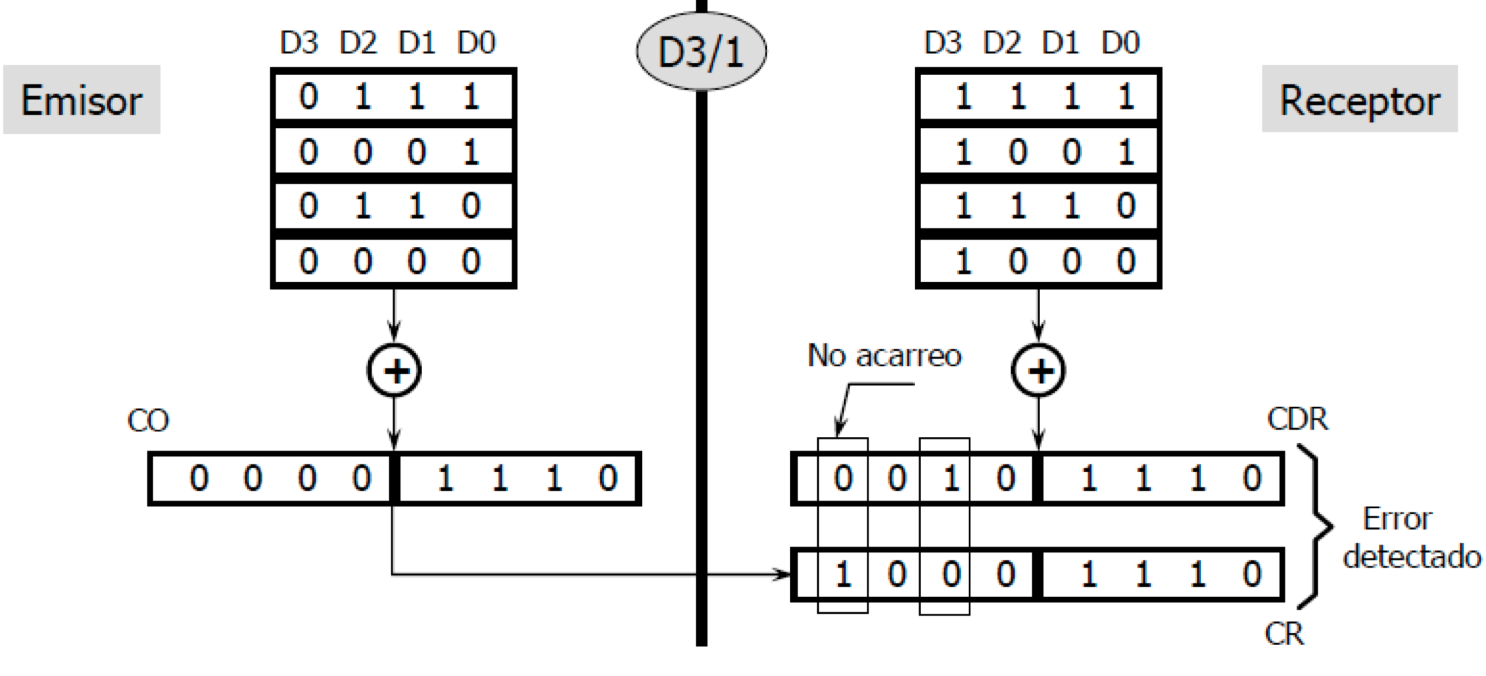
\includegraphics[width=\textwidth]{res/ejemplo_cs}
	\label{ej_cs}
	\caption{Ejemplo checksum}
	\end{figure}

\section{Berger}
redundancia que introduce el código y cobertura del mismo ante diferente tipo de errores

	La redundancia que añade Berger se vuelve insignificante cuando tratamos con cadenas de datos largas (véase Figura \ref{t_berger}), sin embargo, para cadenas cortas inserta demasiada. Además es un código separable, lo que hace muy sencilla su decodificación.
	Lo que se hace para comprobar que la transmisión es correcta es realizar la suma y ver que está bien. Al tratarse de datos binarios, puede darse el caso en el que cambien dos datos y la suma siga dando lo mismo, por lo tanto no se detectaría el fallo. Se muestra un ejemplo en la Figura~\ref{ej_berger}.
	\begin{figure}[h!]
		\centering
		\begin{tabular}{| c | c | c |}
				
			\hline
			
			Código enviado & $\rightarrow$ & Código recibido \\
			\hline
			\rowcolor{LightCyan}
			1001 101 & $\rightarrow$ & 1010 101 \\ 
			\hline
				
		\end{tabular}

		\label{ej_berger}
		\caption{Ejemplo de fallo}
	\end{figure}
	Fallan dos bits pero, como la suma da lo mismo, no se detectaría el fallo.
	\subsection{\emph{Una vez codificado, ¿cuántos bits tiene el código original?}}
	Sabemos que el número de bits que añade Berger es $k = [log_2(I+1)]$ siendo k la longitud de bits añadidos e I la longitud del dato original no codificado. Sin embargo, al decodificar, sabemos que el código codificado tiene longitud $I + k$, es decir, $I + log_2(I+1)$ y, de esta fórmula no se puede despejar I. 
	Por lo tanto, estudio los datos de la Figura \ref{t_berger} para encontrar una relación que me permita conseguir la longitud del dato original a partir del codificado.
	
	\begin{figure}[h!]
		\centering
		\begin{tabular}{| c | c | c |}
				\hline
				Dato original & Añadido & Total \\ \hline
				\rowcolor{LightCyan}
				1 & 1 & 2 \\ \hline
				\rowcolor{LightCyan}
				2 & 2 & 3 \\ \hline
				3 & 2 & 5 \\ \hline
				\rowcolor{LightCyan}
				4 & 3 & 6 \\ \hline
				... & 3 & ... \\ \hline
				7 & 3 & 10 \\ \hline
				\rowcolor{LightCyan}
				8 & 4 & 11 \\ \hline
				9 & 4 & 12 \\ \hline
				... & 4 & ... \\ \hline
				15 & 4 & 19 \\ \hline
				\rowcolor{LightCyan}
				16 & 5 & 20 \\ \hline
				... & 5 &  \\ \hline
				31 & 5 & 36 \\ \hline
				\rowcolor{LightCyan}
				... & 6 & ... \\ \hline
				63 & 6 & 69 \\ \hline
				\rowcolor{LightCyan}
				64 & 7 & 71 \\ \hline
				... & 7 & ... \\ \hline
				\rowcolor{LightCyan}
				128 & 8 & 134 \\ \hline
				... & ... & ... \\ 
				\hline
		\end{tabular}

		\label{t_berger}
		\caption{Tabla de código Berger}
	\end{figure}
	Como se ve en la tabla, cuando el dato original tiene como longitud $2^i$ se añade un nuevo bit a la codificación. Por lo tanto, sólo hay que calcular la potencia de dos a la que corresponde el Total para hallar el número de bits del dato original.

\section{Comparación de los códigos}
	En resumen, los códigos Berger son muy cómodos de usar, por la facilidad de codificación y decodificación. Los que usan checksum, sin embargo, tienen que realizar la suma de todos los elementos y enviarla a mayores, por lo que puede resultar más costoso. Sin embargo, cuando se transmiten datos en grandes bloques, la técnica del checksum funciona bien, ya que suma por bloques y no individualmente.

	Por último, y un factor muy importante en sistemas críticos, el código checksum otorga mayor cobertura que el Berger, por lo que dependiendo de lo que busque nuestro sistema, será más adecuado uno u otro. Si necesitamos alta cobertura usaremos checksum, a pesar de la latencia, sin embargo, si es importante la rapidez del sistema y no se necesita tanta cobertura, nos convendrá un código Berger.
\end{document}
